\documentclass{article}
\usepackage[utf8x]{inputenc}
\usepackage[portuguese]{babel}
\usepackage[margin=2.5cm]{geometry}
\usepackage{float}
\usepackage{graphicx}
\setlength{\parskip}{5mm}
\setlength{\parindent}{0mm}
\linespread{1.2}
\usepackage[usenames,dvipsnames,svgnames,table]{xcolor}
\usepackage{fancyhdr}
\usepackage[symbol]{footmisc}
\usepackage{amsfonts,amsmath,amssymb,amsthm}
\newtheorem{thm}{Teorema}[]
\usepackage{caption}
\usepackage[shortlabels]{enumitem}
\usepackage{verbatim}
\usepackage{listings}
\usepackage[table]{xcolor}
\usepackage{tabu}
\usepackage{array}
\usepackage{tikz}
\usepackage{url}
\def\checkmark{\tikz\fill[scale=0.4](0,.35) -- (.25,0) -- (1,.7) -- (.25,.15) -- cycle;}
\setlength{\parindent}{10mm}
\setlength{\parskip}{1mm}
\makeatletter
\newcommand{\thickhline}{%
    \noalign {\ifnum 0=`}\fi \hrule height 1pt
    \futurelet \reserved@a \@xhline
}
\newcolumntype{"}{@{\hskip\tabcolsep\vrule width 1pt\hskip\tabcolsep}}
\makeatother
\definecolor{codegreen}{rgb}{0,0.6,0}
\definecolor{codegray}{rgb}{0.5,0.5,0.5}
\definecolor{codepurple}{rgb}{0.58,0,0.82}
\definecolor{backcolour}{rgb}{0.95,0.95,0.92}
\lstdefinestyle{mystyle}{
  backgroundcolor=\color{backcolour},   commentstyle=\color{codegreen},
  keywordstyle=\color{magenta},
  numberstyle=\tiny\color{codegray},
  stringstyle=\color{codepurple},
  basicstyle=\footnotesize,
  breakatwhitespace=false,
  breaklines=true,
  captionpos=b,
  keepspaces=true,
  numbers=left,
  numbersep=5pt,
  showspaces=false,
  showstringspaces=false,
  showtabs=false,
  tabsize=2
}
\lstset{style=mystyle}
\title{\textbf{Inteligência Artificial\\Relatório 4 - Redes neuronais}}
\author{\textbf{Grupo 8}\\[4mm]Luís Pinto, nº 201704025\\Sónia Almeida, nº 201811293\\Miguel Lançóis, nº 201506342}
\date{\today}
\begin{document}
\maketitle
\newpage
\tableofcontents
\clearpage
\pagestyle{fancy}
\fancyhf{}
\setlength{\headheight}{30pt}
\rhead{Relatório nº4}
\lhead{\textbf{Grupo 8}}
\setlength{\footskip}{15pt}
\rfoot{\thepage}
\section{Introdução}
\hspace{10mm}Neste trabalho, vamos criar uma rede neuronal composta por duas camadas de neurónios.
\section{Redes neuronais}
\subsection{O que são?}
\hspace{10mm}As redes neuronais são compostas por neurónios e permitem, graças a um conjunto de treino, "aprender". Os neurónios de uma rede neuronal são inspirados por os neurónios presentes na natureza mas o modelo utilizado nas redes neuronais é simplificado já que os neurónios do nosse cérebro não são bem conhecidos. No nosso cérebro, um neurônio é composto por um corpo celular, dendritos e axônios, como se pode ver na figura 1 (retirada do site \url{https://www.researchgate.net/figure/Figura-2-Representacao-esquematica-da-estrutura-do-neuronio-79_fig1_230640478}):


\begin{center} 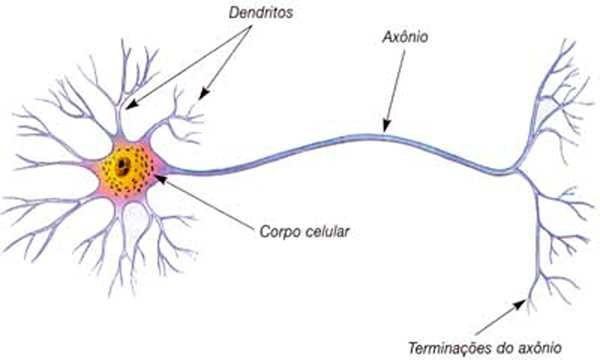
\includegraphics[scale=0.75]{neuronio.png} \end{center}
\begin{center} \textit{\textbf{Fig.1:} neurônio }
\end{center}


 Em redes neuronais, um neurônio é um elemento aritmético simples e uma rede neuronal é um conjunto de neurônios interligados.


\subsection{Neurônio computacional}
\hspace{10 mm} Um neurônio computacional é composto por um conjunto de entradas, que têm um peso associado, por um conjunto de saídas e por uma função de ativação. Cada entrada tem associada um peso aleatório $ w_{i,j} $ (entre -1 e 1 no nosso caso), onde j representa cada link de entrada e i o número do neurônio considerado. Para o neurônio i, deve calcular-se o sumatório das entradas $ a_{j} $ multiplicadas por o peso $ w_{i,j} $ :
 $ \displaystyle { v_{i} = \sum_{j}^{}}  a_{j}  w_{i,j}  $
 O valor da saída $ a_{i}$ do neurônio i é dada por g($v_{i}$) onde g é a função de ativação. No nosso caso, a função de ativação é dada pela seguinte expressão:  $ g(v_{i}) = \frac{1}{1 + e^{-v_{i}}}$.
Esta função é uma sigmoide que é diferenciável, o que é muito importante para poder minimizar o erro de classificação durante o treinamento da rede. A função de ativação de ve permitir a comparação entre a entrada e a saída e depende então dos dados.

\subsection{Tipos de redes neuronais}
Exitem vários tipos de redes neuronais:
\begin{itemize}
  \item[\textbullet]{feed-forward: não há ciclos, o grafo é direcionado e os links são unidirecionais. Não há links entre neurônios da mesma camada. Dados que os links são unidirecionais, a informação não retorna para os nós das camadas anteriores.}
  \item[\textbullet]{recorrente: os links podem formar topologias arbitrárias.}
  \item[\textbullet]{Hopfield: as conexões são bidirecionais entre os nós com pesos simétricos. Todos os nós podem ser entrada ou saída. A função de ativação produz -1 ou +1. Não encontra ótimos globais.}
  \item[\textbullet]{Máquinas de Boltzmann: também usa pesos simétricos mas inclui unidades (escondidas) que não são nem entrada nem saída. A função de ativação é estocástica, onde a probabilidade de ser 1 é função dos pesos da entrada.}
\end{itemize}
No nosso caso, são Perceptrons que vão ser usados. Os perceptrons são o exemplo mais simples de redes feed-forxard com apenas uma camada.

\subsection{Multi Layer Perceptrons (MPR)}
\hspace{10 mm} Multi Layer Perceptrons são Perceptrons de várias camadas. Neste trabalho, vamos usar um MPR com duas camadas. No nosso modelo, os neurônios de uma camada só estão ligados a neurônios de outra camada e não a neurônios da mesma camada:

\begin{center} 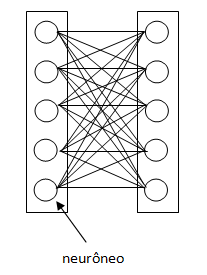
\includegraphics[scale=0.75]{perceptron.png} \end{center}
\begin{center} \textit{\textbf{Fig.2:} rede de perceptron }
\end{center}

Os pesos são atualizados com a seguinte fórmula:
$w^{(k+1)} = w^{(k)} + \lambda \lfloor v_{i} - g(w^{k},a_i) \rfloor a_i$
onde $w^{(k)}$ representa o peso para uma dada entrada do neurônio $i$ ao instante $k$.

\section{Algoritmo de redes neuronais}
\hspace{10 mm}Para saber se o nosso modelo funciona bem, de vemos utilizar um conjunto de treino e outro de teste.

\section{Implementação}
\textbf{Linguagem:} Para a implementação do código decidimos utilizar a linguagem \textit{Python 3.7}.\\[2mm]
\textbf{Estrutura de Dados:}
\section{Resultados}
\textbf{Execução dos testes:}
\begin{itemize}
  \item[\textbullet]{Executámos iterações até termos um erro inferior a 0.05, ou até obter $10^6$ iterações;}
  \item[\textbullet]{Testámos vários learning rates diferentes e, para cada um deles, testámos 4 inputs exemplos diferentes: 1111,1010,0011,0111;}
  \item[\textbullet]{Verificámos qual dos 4 exemplos obteve o maior erro e considerámos esse o erro para a nossa tabela de resultados.}
\end{itemize}
\textbf{Testes:}
\begin{center}
\begin{tabular}{|c|c|c|c|}
  \hline
  \textbf{Learning Rate} & \textbf{Número de Iterações} & \textbf{Erro} & \textbf{Tempo de execução (ms)}\\
  \hline
  0.05 & 999999 & 0.200313 & 120793 \\
  \hline
  0.10 & 247659 & 0.049998 & 29223\\
  \hline
  0.15 & 297898 & 0.049998 & 35058 \\
  \hline
  0.20 & 84830 & 0.049991 & 10004 \\
  \hline
  0.25 & 228214 & 0.037433 & 27106\\
  \hline
  0.30 & 331040 & 0.049970 & 38869\\
  \hline
  0.35 & 329790 & 0.049958 & 38211\\
  \hline
  0.40 & 999999 & 0.800029 & 116724\\
  \hline
  0.45 & 999999 & 0.750028 & 117297\\
  \hline
\end{tabular}
\end{center}
\section{Conclusão}
\hspace{10mm}Ao avaliar cuidadosamente os resultados que obtivemos relativamente aos 4 exemplos referidos na secção 5, determinámos que um learning rate entre 0.20 e 0.25 fornece resultados significativamente mais concretos do que qualquer outro valor do learning agreement. Para além dos resultados apresentados neste relatório, testámos com mais neurónios "fantasma", com nove, e os resultados foram semelhantes. Decidimos ocultar esses testes do relatório uma vez que não nos foi pedido tal tipo de teste mas estes podem ser encontrados no ficheiro \textit{testes.txt} na parte dos testes com 9 neurónios fantasma.
\section{Bibliografia/webgrafia}
\begin{itemize}
  \item{\url{https://artint.info/2e/html/ArtInt2e.Ch7.S5.html}}
  \item{\url{http://www.dcc.fc.up.pt/~ines/aulas/1718/IA/neunets.pdf}}
\end{itemize}
\end{document}
